\documentclass{article}
\usepackage{tikz}

\begin{document}

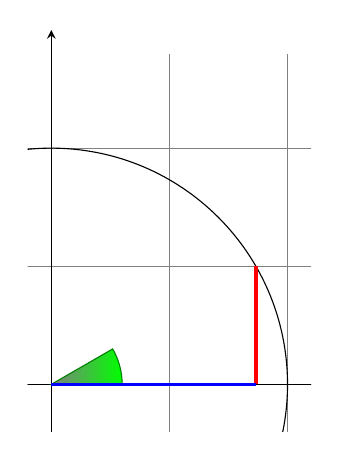
\begin{tikzpicture}[>=stealth, scale=3]                         % Stealth is a type of arrow 
    \clip (-0.1, -0.2) rectangle (1.1,1.51);
    \draw[step=.5cm,gray,very thin] (-1.4,-1.4) grid (1.4,1.4);
    \draw[<->](-1.5, 0) -- (1.5,0);
    \draw[<->](0, -1.5) -- (0, 1.5);
    \draw (0,0) circle [radius=1cm];
%    \draw (0,0) rectangle(0.5,0.5);
%    \draw (-0.5,-0.5) rectangle(-1,-1);
%    \draw (3mm,0mm) arc [start angle=0, end angle=30, radius=3mm];
%    \filldraw[fill=green!20!white, draw=green!50!black] (0,0) -- (3mm,0mm)
%        arc [start angle=0, end angle=30, radius=3mm] --cycle;
%    \fill[green!20!white] (0,0) --(3mm, 0mm)
%            arc [start angle=0, end angle=30, radius=3mm] --cycle; %-- (0,0);
    \shadedraw[left color=gray, right color=green, draw=green!50!black]
    (0,0) -- (3mm,0mm)
    arc [start angle=0, end angle=30, radius=3mm] --cycle;
    \draw[red, very thick] (30:1cm) -- +(0,-0.5);
    \draw[blue, very thick] (30:1cm) ++(0,-0.5) -- (0,0);
    
    
%    \path [name path=upward line] (1,0) -- (1,1);
%    \path [name path=sloped line] (0,0) -- (30:1.5cm);
%    \draw [name intersections={of=upward line and sloped line, by=x}]
%            [very thick, orange]  (1,0) -- (x);

%    \draw (-1,0) .. controls (-1,0.555) and (-0.555,1) .. (0,1)
%                  ..  controls (0.555,1) and (1,0.555) .. (1,0);

\end{tikzpicture}


\end{document}

